%%%%%%%%%%%%%%%%%%%%%%%%%%%%%%%%%%%%%%%%%%%%%%%%%%%%%%%%%%%%%%%%%%%%%%%%%%%%%%%%
%2345678901234567890123456789012345678901234567890123456789012345678901234567890
%        1         2         3         4         5         6         7         8

\documentclass[letterpaper, 10 pt, conference]{ieeeconf}  % Comment this line out
                                                          % if you need a4paper
%\documentclass[a4paper, 10pt, conference]{ieeeconf}      % Use this line for a4
                                                          % paper

\IEEEoverridecommandlockouts                              % This command is only
                                                          % needed if you want to
                                                          % use the \thanks command
\overrideIEEEmargins
% See the \addtolength command later in the file to balance the column lengths
% on the last page of the document



% The following packages can be found on http:\\www.ctan.org
%\usepackage{graphics} % for pdf, bitmapped graphics files
%\usepackage{epsfig} % for postscript graphics files
%\usepackage{mathptmx} % assumes new font selection scheme installed
%\usepackage{times} % assumes new font selection scheme installed
%\usepackage{amsmath} % assumes amsmath package installed
%\usepackage{amssymb}  % assumes amsmath package installed
%\usepackage{hyperref}

\title{\LARGE \bf
Extending Main-Memory Persistent File Systems for NVM to support high volume data storage using disks
}

%\author{ \parbox{3 in}{\centering Huibert Kwakernaak*
%         \thanks{*Use the $\backslash$thanks command to put information here}\\
%         Faculty of Electrical Engineering, Mathematics and Computer Science\\
%         University of Twente\\
%         7500 AE Enschede, The Netherlands\\
%         {\tt\small h.kwakernaak@autsubmit.com}}
%         \hspace*{ 0.5 in}
%         \parbox{3 in}{ \centering Pradeep Misra**
%         \thanks{**The footnote marks may be inserted manually}\\
%        Department of Electrical Engineering \\
%         Wright State University\\
%         Dayton, OH 45435, USA\\
%         {\tt\small pmisra@cs.wright.edu}}
%}

\author{Aishwarya Ganesan, Saket Saurabh, Siddharth Suresh, Udip Pant\\
\{ag, ssaurabh, ssuresh6, upant\}@cs.wisc.edu\\
University of Wisconsin-Madison
}


\begin{document}


\maketitle
\thispagestyle{empty}
\pagestyle{empty}


%%%%%%%%%%%%%%%%%%%%%%%%%%%%%%%%%%%%%%%%%%%%%%%%%%%%%%%%%%%%%%%%%%%%%%%%%%%%%%%%
\begin{abstract}

Fast non-volatile memories (NVM) are byte addressable, offer latencies close to DRAM and have densities better than DRAM that allow applications to persist their data close to memory latencies, but at a higher predicted cost per byte. The I/O latency of a disk-based filesystem is higher than a pure memory-based filesystem, but memory-based filesystems are limited by their storage cost. We propose a hybrid approach, where we use NVM as a primary storage and use flash/disk-based for secondary storage. Our approach is to combine the low latency of NVM and low cost of disk-based storage without regressing on the performance and still offer similar consistency guarantees. 

\end{abstract}


%%%%%%%%%%%%%%%%%%%%%%%%%%%%%%%%%%%%%%%%%%%%%%%%%%%%%%%%%%%%%%%%%%%%%%%%%%%%%%%%



\section{INTRODUCTION}

Most modern systems have been built with the disk or SSDs as the persistent storage medium and the DRAM for temporary fast byte-addressable memory usage. The data that resides in volatile memory can be lost on crashes or power failure. Moreover, with the emergence of modern storage technologies and new byte addressable persistent memory technologies which offer much lower write and read latencies compared to flash memory at a slightly higher cost, it is imperative that future systems would move towards the usage of byte-addressable non volatile memory as the primary storage with the disk as the secondary storage medium. In this paper we have implemented and evaluated one such system. There has always been a trade-off between data durability and data read/write performance when deciding between a fast, volatile storage medium like DRAM versus a slow, persistent storage medium like disk. Persistent memory technologies like phase change spin-torque transfer RAM (STT-RAM), phase change memory (PCM), resistive RAM (ReRAM), and 3D XPoint memory technology can solve both of these problems[Suzuki].\\

One of the earliest file systems to be proposed for non-volatile memory systems was the byte-addressable persistent file system (BPFS) [BPFS] by a group of researchers working at Microsoft Research. The BPFS paper showed that simply running a disk-based traditional file system on top of persistent memory is not enough to provide high performance. BPFS proposes adding two new hardware primitives- 8-byte atomic writes and epoch barriers- to enforce atomicity and write ordering. It also proposed to modify the file system data structure to a new tree-based data structure  could support in-place updates. A new technique called short-circuit shadow paging as a copy-on-write mechanism. BPFS achieves fine-grained access to persistent data at a much improved performance, while at the same time providing strong reliability and safety guarantees. \\

The primary focus of this paper is to examine the benefit of such a multi-tiered storage hierarchy consisting of NVRAM and Disk or Flash on File Systems. The Paper "Better I/O Through Byte-Addressable, Persistent Memory" examined the implementation of a new file system for BPRAM called BPFS which performed faster than any other file system designed of block based storage devices. But the BPFS[] paper does not consider the fact that the relatively high cost/byte of NVM could hinder such a filesystem from being pervasively used since commodity systems will not have sufficient non volatile memory storage.\\

Due to the inability to store all data blocks in NVRAM, we have explored the usage of Anti-Caching [Paper] in BPFS.Anti-caching entails the storage of the more frequently accessed data blocks in the persistent byte addressable memory while storing the rest of the blocks on disk or flash memory. In short, while trying to read a disk block, the file system first checks to see if the block is already in the NVRAM and fetches the block from disk and evicts blocks from NVRAM to make room for the new block if needed using an LRU policy. Since double buffering of blocks is a waste of resourcs, the usage of NVRAM as a persistent store also requires us to pin certain blocks and maintain an eviction policy between itself and the secondary storage device. \\

The primary motivation for building such a system is to come up with a flexible design that scales itself well irrespective of the size of the storage tier, i.e capacity of NVRAM and capacity of disk or flash. This approach is very similar to the virtual memory swapping in operating systems wherein when the amount of data exceeds available memory, cold blocks are written to disk giving an impression to the file system that the amount of memory in NVM is infinite but at the same time provides the best possible performance with the amount of NVM available. This has been achieved through the use of anti-caching. 


\section{BACKGROUND}
In this section, we will briefly discuss the relevant background on BPFS, a file system for byte address persistent memory. BPFS is one of the earliest file systems to be proposed for non-volatile memory systems and the authors showed that simply running a disk-based traditional file system on top of persistent memory is not enough to provide high performance. We will first introduce the BPFS file system layout and also discuss why the design is limited in terms of the cost of storage and volume of storage. We will also briefly describe the techniques proposed in BPFS to achieve consistency and how they achieve atomicity and write ordering. We then describe the changes made to the persistent data structures and file system code to support a disk backed secondary storage in a subsequent section.



\subsection{BPFS Layout}
BPFS stores all the file system metadata and data in the form of a tree structure consisting of fixed-size blocks of 4KB in the non-volatile memory. The BPFS file system consists of three kinds of files namely inode file, directory file and data file with each of these inturn arranged as a tree. The inode file is represented by a tree structure with the root of the inode file serving as the root of the file system. The location of this root node is stored at a known location in the non-volatile memory. Each of the leaves in the inode file contain an array of inode structures with each inode structure representing either a file or a directory. This inode structure contain the pointer to the root of the file or directory that the inode represents.

\subsection{Anti-Cache Manager}

Non Volatile Memory (NVM) is the primary data store and it also contains the more frequently accessed blocks, which is referred to as "hot data". But since the capacity of the persistent NVM is limited, we have used the concept of Anti-Caching [Refer Paper here] to periodically evict blocks from the NVM to the disk periodically based on an eviction policy. The eviction policy thus used in this design is the Least Recently Used (LRU) policy. The Anti-Cache Manager keeps track of all the blocks that are written to the NVM and periodically evicts blocks when the number of blocks in the NVM exceeds a pre-determined threshold, which is used to ensure that the NVM is always available from writing blocks, which has helped us drastically reduce our write latency for blocks. \\

In order to achieve this, the anti-cache manager runs as a separate background thread which continuously probes the NVM and performs silent eviction. In order to ensure that data blocks that are currently being evicted to disk do not get updated by the file system, a block level locking mechanism is used which implicitly prevents any updates to the block currently being evicted. The performance impact of the locking was found to be negligibe in the FileServer and Varmail macro benchmarks. 


\subsection{Disk Manager}

The Disk Manager component simulates a virtual disk through of a file stored on disk in the BPFS partition of predetermined size. It exposes APIs for reading and writing blocks into the disk individually and in bulk. It performs prefetching of additional blocks when a read is performed. The liefetime of the prefetched blocks in memory is predetermined to ensure that unused prefetched blocks are cleaned up regularly with the help of a background thread. To avoid fragmentation, a free list of blocks that have been freed is maintained. Since the disk manager writes blocks into a file, the buffer cache is used to buffer writes until all the blocks are written into the file. Our current implementation provides consistency at the expense of performance by notifying BPFS after persisting the blocks, which inturn updates the indirect pointer in the inodes to point to the new blocks thorugh a blocking call. \\

The disk manager also exposes another write API to the Anti-Cache Manager to facilitate writing one block at a time, for faster random writes since any free block on disk can be used for writing and does not require sequential locality. To furher improve performance in the case of bulk eviction of blocks from the anti-cache manager, the disk manager performs an explicit flush only after writing all the blocks on to the disk.\\

\section{File System Operations}

\subsection{Read}


When a read operation is performed on a file, the BPFS crawls the inode tree to the indirect block containing the pointer to the data block, identifies the location of the data block using the MSB which indicates whether the block is on disk or in NVM, then fetches the block into memory and asynchronously writes it back into NVM. Once the block is persisted in NVM, it frees the block on disk and updates the indirect pointer in the inode tree to point to the new block location in NVM atomically.

When a read operations is performed on a directory, the BPFS crawls the inode tree and the directory file blocks are loaded into memory from NVM and the necessary updates are made into the directory entry cache. It then traverses all the necessary inodes in the directory file and reads them from NVM.
 
\subsection{Write}

When a write operation is performed on a file, the BPFS traverses the inode tree to find the indirect block containing the pointers to the data block of the fle and identifies the location of the data blocks. If the data block is in NVM, the write operation is performed in-place and has no additional overhead. If the data block is on disk, the block is fetched into NVM thus performing a copy on write of the data block and this block is updated and written back to NVM. The block on disk is then freed and the control comes back to the BPFS crawler. The indirect pointer in the inode tree is then updated to point to this new block location in-place along with in-place writes of the other internal nodes. The inode access time is also updated through an in-place atomic write.


\subsection{Open}

When a file is opened, the directory inode tree is parsed to find the file. If the file is not found and a create is requested, a new new inode nunber is generated and the new inode is written to the inode file. Then the directory file is then updated. All these updates are performed in place. Since the metadata updates are in-place and in NVM, they are faster than usual disk writes and the additional overhead of metadata journaling can also be avoided by avoiding disk writes.



\subsection{File system Consistency}

\section{DESIGN}

\begin{figure}
\centering
\vspace{-0.2in}
%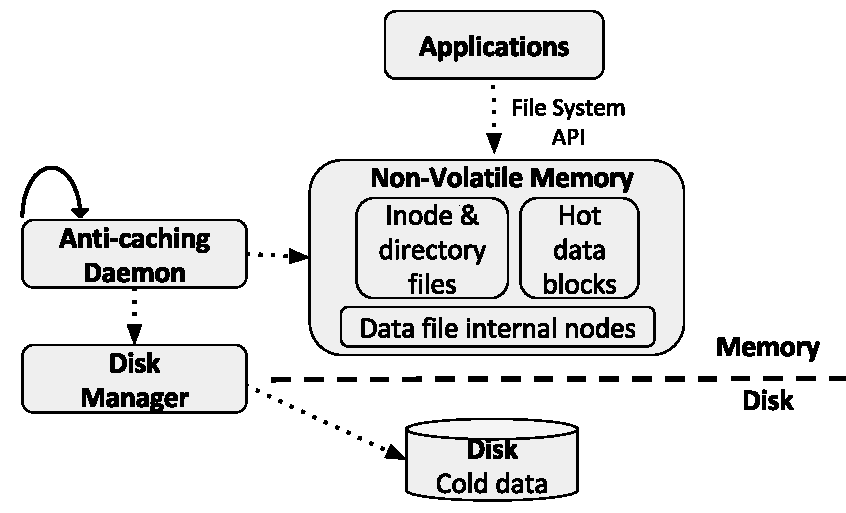
\includegraphics{bpfs.pdf}
\vspace{-0.1in}
%\mycaption{fig-bpfs}{Architecture}
\end{figure}

\section{Evaluation}

We compare the performance of this system with that of BPFS and ext4 file systems to evaluate its design and implementation. We use the performance of BPFS as a baseline and focus on following key questions:
\begin{itemize}
\item What is the cost and overhead of the anti caching mechanism on top of the BPFS system?
\item How does the degree of hotness and coldness of stored data affect the performance of the system?
\item How does this file system perform for different cache eviction threshold? (Improve this)
\end{itemize}

\subsection{Method}
Making a meaningful performance comparison of this system with both the memory based file system such as BPFS and the disk based file system such as ext4 presents presents challenges at different levels. We cannot make comparison in isolation since our implementation is a hybrid approach that incorporates both systems. Another difficulty is that for a disk based file systems, such as ext4 that runs in the kernel layer, several parameters and behaviors are opaque to users and we have very limited contol on enforcing the pure disk-based behaviors. For instance, ext4 filesystems performs several operations in memory and commit to the disk only periodically [cite{something}]. 

For the purpose of the evaluation, we run our experiments on a real hardware with 8 CPU cores running RedHat Linux Operating Systems with 16 GM of memory, 500 GB of Solid state Drive and * MB cacheline. We simulate the behavior of NVM on the DRAM due to unavailability of the hardware (really???). Unless otherwise noted, both the original and our implementation of BPFS are mounted in the memory with 2 GB image. The anticaching daemon is set to run at 10 ms by default with caching occupancy threshold of 40 MB. These values were chosen by performing emperical analysis.    

\subsection{Experimental evaluations}
In this section we present the experimental evaluations of this file system using differnt micro and macro benchmarks and throughput evalations and offer comparisons with those of BPFS and ext4 file-systems. 

\subsubsection{Microbenchmarks}


\section{RELATED WORK}

There has always been a trade-off between data durability and data read/write performance when deciding between a fast, volatile storage medium like DRAM versus a slow, persistent storage medium like disk. Persistent memory technologies like phase change spin-torque transfer RAM (STT-RAM), phase change memory (PCM), resistive RAM (ReRAM), and 3D XPoint memory technology can solve both of these problems\cite{c9}.

Researchers have proposed various interfaces and programming models \cite{c4,c6} to simplify persistent memory programming and libraries that ensure consistency in the presence of failures. Mnemosyne \cite{c6} allows applications to have persistent regions in address space that survive crashes. It provides support for one word atomic updates and lightweight transactions for consistent updates to persistent memory data structures. Mnemosyne handles the case where NVM runs out of space and this is closely related to our work, since our primary assumption is that NVM memory is limited.

Conventional file systems have been optimized for disk and maintaining disk based consistency. Maintaining consistency in memory based systems is different and is still a challenge. One of the earliest file systems to be proposed for non-volatile memory systems was the byte-addressable persistent file system (BPFS) \cite{c10}. The BPFS paper showed that simply running a disk-based traditional file system on top of persistent memory is not enough to provide high performance. BPFS proposes adding two new hardware primitives- an 8-byte atomic write primitive and an epoch barrier primitive- to enforce atomicity and write ordering. It also proposed to modify the file system data structure to a new tree-based data structure that could support in-place updates. A new technique called short-circuit shadow paging as a copy-on-write mechanism has been proposed. BPFS achieves fine-grained access to persistent data at a much improved performance, while at the same time providing strong reliability and safety guarantees. 

NOVA \cite{c8} takes a different approach and implements a log structured file system that provides better concurrency by using separate logs for each inode and guarantees consistency by storing the journals in NVM. The overhead of garbage collection in LFS is also reduced in NOVA by exploiting the low random write latency of NVM when compared to the poor sequential write access latencies of SSDs and disks.

PMFS \cite{c3} is similar to other persistent memory file systems but provides transparent large page support for faster memory-mapped I/O and provides a way for applications to specify file sizes hints causing PMFS to use large pages for file’s data nodes. Aerie \cite{c5} provides a flexible file system architecture that aims to avoid the overhead of trapping into kernel while reading or writing to a file. It achieves this by splitting the functionality across different layers - a kernel layer that handles protection, allocation and addressing, a user library that directly accesses NVM for file reads, file writes and metadata reads, and a trusted service that coordinates updates to metadata.  

The Bankshot paper\cite{c7} provides the motivation for building a user level library that intercepts the read/write system calls and a caching architecture for faster memories like NVM to ensure that the software overhead of caching would be low. Bankshot minimizes cache hit latency by allowing applications to access the cache hardware without operating system intervention. The previous SSD based caching systems used an OS level Cache Manager, which tracks dirty data and maintains a mapping between caching locations and the backing store. The concepts used in Backshot helps reduce latency in the case of a Cache Hit, which is interesting to explore. Since the Bankshot cache library has been implemented in the user space, some of the implementation ideas used in this paper for cache eviction and cache recovery is also being explored and evaluated. 
 
The current research around file systems for NVM is focused on maximizing file system performance by exploiting higher I/O throughput guarantees of the byte-addressable persistent NVM \cite{c10,c8,c3,c5}. While a majority of the research in this area has tried to solve the problem of consistency, write ordering and atomicity associated with implementing file systems for NVM, there has been some related work in accelerating the performance of existing file systems using NVM \cite{c11, c12}. We borrow the idea of Anti-Caching \cite{c13} from the database community and propose a radical new approach to file system design in context of main-memory file systems like BPFS \cite{c10}, \cite{c8}, where NVM is used as a primary data store for ‘hot’ data and the disks serve as a backing store for ‘cold’ data. While these file systems for NVM have been proposed as a replacement for traditional disk and flash-based file systems, our work proposes to enhance these file systems to function alongside the existing traditional disk and flash-based file systems. 

Ghandeharizadeh et. al. \cite{c2} propose a way to use knowledge about the frequencies of read and write requests to individual data items in order to determine the optimal cache configuration given a fixed budget. It employs an offline optimal algorithm that computes: (1) the choice and sizes of the stashes that constitute a cache given a fixed budget and (2) a static placement of data items across the stashes. This paper considers both tiering and replication of data across the selected choices of storage media. Our approach is different in following ways- we only consider tiering approach and do not replicate data across the storage layers, and the decision of placement of data is done online based on the information such as available space in NVM, size of the data and last access time. A separate background process moves “cold” data from higher storage level (NVM) to lower level (SSD / disk). 

Lv et. al. \cite{c1} propose a strategy named Hotness Aware Hit (HAT) for efficient buffer management in flash-based hybrid storage systems by dividing pages into three hotness categories: hot, warm and cold. In general, the hot, warm and cold pages are kept in main memory, flash and hard disk respectively. They employ a page reference queue to record the page reference history. Based on the reference information, the pages are marked with different hotness levels. Pages are allocated to different levels in the storage hierarchy according to the page access sequence and pages’ hotness. Our approach employs a similar strategy to determine the hotness of data and adapts it with the changes in the usage pattern by employing a multi-tier page reference history. However, our approach differs from this work because we do not use NVM merely for buffering of data. We use it as one of the storage devices in the multi-tier storage system with strategies to make placement decision during the runtime. 
 
\begin{thebibliography}{99}

\bibitem{c11} Baker, M., Asami, S., Deprit, E., Ouseterhout, J. and Seltzer, M., 1992, September. Non-volatile memory for fast, reliable file systems. In ACM SIGPLAN Notices (Vol. 27, No. 9, pp. 10-22). ACM.

\bibitem{c7} Bhaskaran, M. S., Xu, J., Swanson, S. (2014). Bankshot: Caching slow storage in fast non-volatile memory. ACM SIGOPS Operating Systems Review, 48(1), 73-81.	

\bibitem{c12} Chen, J., Wei, Q., Chen, C. and Wu, L.F., 2013, April. A file system metadata accelerator with non-volatile memory. In Proceedings of Symposium on Mass Storage Systems and Technologies, Monterey, CA, USA (pp. 19-20).

\bibitem{c10} Condit, J., Nightingale, E. B., Frost, C., Ipek, E., Lee, B., Burger, D.,  Coetzee, D. (2009, October). Better I/O through byte-addressable, persistent memory. In Proceedings of the ACM SIGOPS 22nd symposium on Operating systems principles (pp. 133-146). ACM.

\bibitem{c13} DeBrabant, Justin, Andrew Pavlo, Stephen Tu, Michael Stonebraker, and Stan Zdonik. "Anti-caching: A new approach to database management system architecture." Proceedings of the VLDB Endowment 6, no. 14 (2013): 1942-1953.

\bibitem{c3} Dulloor, S. R., Kumar, S., Keshavamurthy, A., Lantz, P., Reddy, D., Sankaran, R., Jackson, J. (2014, April). System software for persistent memory. In Proceedings of the Ninth European Conference on Computer Systems (p. 15). ACM.

\bibitem{c2} Ghandeharizadeh, S., Irani, S., Lam, J. (2015). Memory Hierarchy Design for Caching Middleware in the Age of NVM.

\bibitem{c1} Lv, Y., Cui, B., Chen, X., Li, J. (2013, October). Hotness-aware buffer management for flash-based hybrid storage systems. In Proceedings of the 22nd ACM international conference on Conference on information and knowledge management (pp. 1631-1636). ACM.	

\bibitem{c4} Persistent Memory Programming. http://pmem.io/nvml/

\bibitem{c9} Suzuki K. and Swanson S. The Non-Volatile Memory Technology Database (NVMDB). Technical Report CS2015-1011, Department of Computer Science and Engineering, University of California, San Diego, May 2015. http://nvmdb.ucsd.edu.

\bibitem{c5} Volos, H., Nalli, S., Panneerselvam, S., Varadarajan, V., Saxena, P., Swift, M. M. (2014, April). Aerie: Flexible file-system interfaces to storage-class memory. In Proceedings of the Ninth European Conference on Computer Systems (p. 14). ACM.

\bibitem{c6} Volos, H., Tack, A. J., Swift, M. M. (2011). Mnemosyne: Lightweight persistent memory. ACM SIGPLAN Notices, 46(3), 91-104.	

\bibitem{c8} Xu, J., Swanson, S. NOVA: A Log-structured File System for Hybrid Volatile/Non-volatile Main Memories.

\end{thebibliography}

\end{document}
